\section*{Summary of the Proposal}

This project builds a small MLIR-based framework that acts as a dialect to describe kernels and their scheduling choices and automatically generate multiple optimized implementations of the same computation. These implementations will be executed on a cluster to measure performance and scaling behavior, enabling systematic study of how scheduling decisions affect HPC workloads.

\section*{Background}

High-performance programs depend heavily on how computations are scheduled and optimized by the compiler, such as how loops are organized, how memory is accessed, and how work is parallelized. Modern compiler infrastructures like LLVM and MLIR are widely used in industry and research to transform high-level programs into efficient machine code, but the optimization process is complex and difficult to experiment with directly. This project proposes to build a small experimental framework on top of MLIR that allows different scheduling choices for a kernel to be expressed explicitly and automatically generated into multiple executable variants. These variants will be run on a small computing cluster to measure performance and scaling behavior. The goal is to create a simple, reproducible way to study how compiler-level scheduling decisions affect real HPC performance.

\section*{Goal and Objectives}

The objective of this project is to build a small prototype framework using MLIR that separates the description of a computation from its scheduling decisions. For a selected kernel family, the framework will allow scheduling parameters such as tile size, loop ordering, and vector width to be specified explicitly. From a single kernel description, the system will automatically generate multiple executable versions with different schedules. These versions will be run on a small cluster to measure runtime, scalability, and efficiency. The project will focus on simplicity and reproducibility rather than building a large or general-purpose system.

\section*{Methods}

The project will be divided in four different stages in the following order:

\begin{enumerate}
\item Kernel baseline implementations will be created for validation. 
\item Minimal representation will be designed in MLIR to describe the kernel and a small set of scheduling parameters. 
\item A prototype compiler pipeline will then translate this representation into executable code. 
\item Performance data will be collected and analyzed to observe trends and tradeoffs.
\end{enumerate}

\subsection*{Hardware Platform}
This proposal is still in an exploratory stage. The current plan is oriented toward multi-core CPUs, as this aligns naturally with the scheduling choices under consideration (tile size, loop order, and vector width). However, I am inclined toward a GPU-only approach given its relevance to modern HPC. Both the specific scheduling decisions and the performance metrics to be collected may change depending on the final hardware platform, this would also depend on the hardware available, regardless both options seem to be reasonable for the scope of this project.

\section*{Kernel Base Implementations}

\subsection*{General Matrix Multiply (GEMM)} 

GEMM is one of the most important kernels in scientific computing, machine learning, and high-performance computing. Its performance is highly sensitive to scheduling decisions such as tile size, loop order, and vector width because these choices determine how well data is reused in cache and how effectively the CPU uses SIMD instructions. GEMM is chosen because it is well understood, easy to validate for correctness, and a standard benchmark for studying performance and compiler behavior.\\

\subsection*{2D Stencil} 

A 2D stencil updates each point in a grid based on its neighbors (for example, averaging surrounding cells). This pattern appears in simulations, fluid dynamics, and image processing. Stencil performance depends strongly on tile size, loop order, and how work is parallelized, since these choices affect memory locality and cache reuse. The 2D stencil is chosen because it represents a classic memory-bound HPC workload and clearly exposes the impact of scheduling decisions on cache behavior and parallel scaling.

\section*{Scheduling Choices}

Now that we have defined the kernel families that will be utilized, we will choose a small example of scheduling choices that will act as our experiment to measure the tradeoffs in performance, I have picked three for each the GEMM and 2D stencil family, these are based on their relevance and the impact they have on performance.

\subsection*{GEMM}
\begin{itemize}
    \item Tile Size
    \item Loop Order
    \item Vector Width
\end{itemize}

\subsection*{2D Stencil}
\begin{itemize}
    \item Tile Size
    \item Loop order
    \item Parallelization: tile-parallel vs row-parallel
\end{itemize}


\section*{MLIR representation}

A minimal representation will be designed in MLIR to describe the chosen kernel and a small set of scheduling parameters. This representation will clearly separate what the computation is from how it is executed. By keeping this representation simple and focused, the framework will allow multiple execution schedules to be generated automatically from the same kernel description while remaining easy to understand, modify, and analyze.

\noindent Below is an example of the commands created through MLIR on the PEAK project, this allow special scheduling choices, similar to what we plan to achieve with our own scheduling choices.

\begin{figure}[H]
\centering
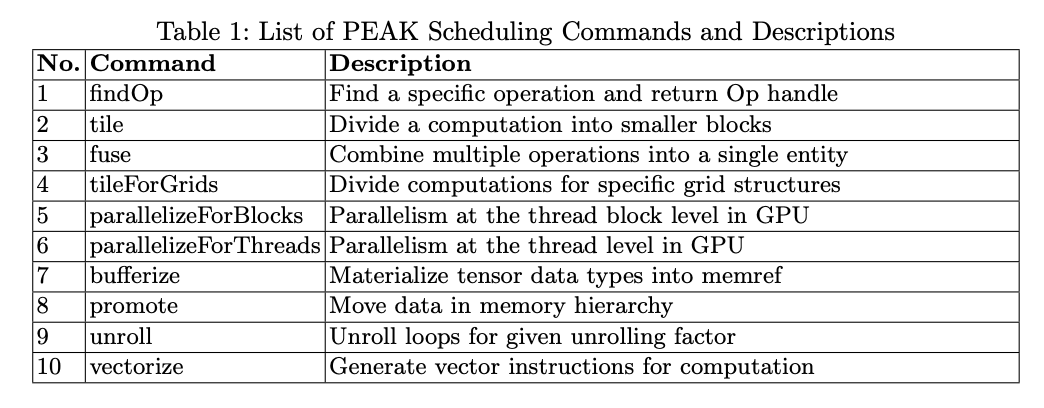
\includegraphics[width=0.6\textwidth]{commands.png}
\end{figure}

\section*{Compiler Construction}

As discussed, we are building a dialect on top of MLIR to make scheduling decisions explicit, and to do so we nee to create a compiler pipeline. The following figure shows an example of how this compiler pipeline might look like. This is an example from the PEAK project.
\noindent Below is an example from the PEAK project of how the MLIR dialect may look like as scheduling commands.

\begin{figure}[H]
\centering
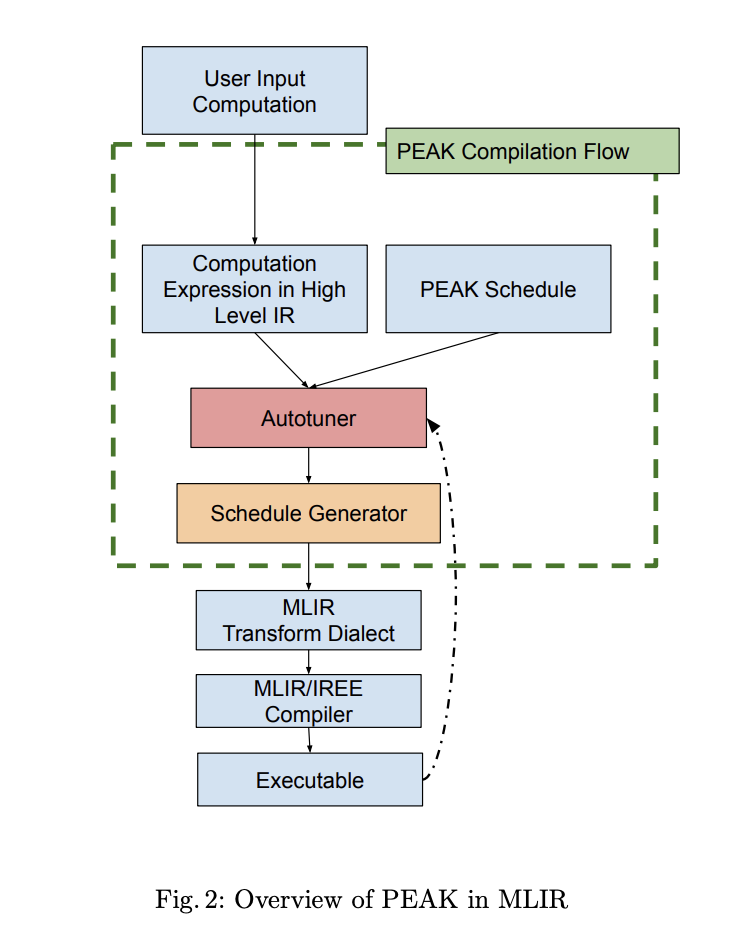
\includegraphics[width=0.5\textwidth]{compiler.png}
\caption{\label{fig:compiler}Overview of the PEAK MLIR.}
\end{figure} 

\section*{Metrics}
The following are the different performance metrics that will be measured to understand the tradeoffs between the different scheduling choices from the kernel families, with this data we will be able to retrieve the conclusions of the project.  

\subsection*{Execution time}
 For each kernel variant and problem size, we will measure wall-clock time of the kernel region (excluding initialization and I/O) using high-resolution timers. Results will be reported as median/mean over multiple runs to reduce noise from OS jitter and system load.
 
\subsection*{Scalability}
 We will evaluate scaling with fixed problem size while increasing thread count (e.g., 1, 2, 4, 8 threads per node).

\subsection*{Compute Efficiency}
To interpret performance beyond runtime, we will compute:

\begin{itemize}
\item Achieved FLOP rate (GFLOP/s) for GEMM using the known operation count.
\item Achieved memory bandwidth (GB/s) for the stencil using known bytes moved.
\end{itemize}
 
\subsection*{Hardware-Level Behavior (Cache / Memory / SIMD).}
 Where supported by the cluster, we will collect hardware performance counter metrics to explain performance differences between schedules, including:
\begin{itemize}
    \item Cache misses / miss rates
    \item Cycles and instructions (CPI/IPC)
    \item Vector/SIMD utilization indicators
\end{itemize}

\cite{lattner2021mlir}
\cite{tavakkoli2023peak}
